\documentclass[smallextended]{svjour3}
\usepackage[utf8]{inputenc}
\usepackage[T1]{fontenc}
\usepackage{graphicx}
\usepackage{amsmath,amssymb}
\usepackage{booktabs}
\usepackage{xcolor}
\usepackage{listings}
\usepackage{hyperref}
\usepackage{url}
\usepackage{enumitem}
\usepackage{float}

\hypersetup{colorlinks=true, linkcolor=blue!60!black, citecolor=blue!60!black, urlcolor=blue!60!black}

\definecolor{codebg}{RGB}{245,245,245}
\definecolor{codeframe}{RGB}{220,220,220}
\lstdefinestyle{bunstyle}{
  backgroundcolor=\color{codebg},
  frame=single,
  rulecolor=\color{codeframe},
  basicstyle=\ttfamily\footnotesize,
  keywordstyle=\color{blue!65!black}\bfseries,
  commentstyle=\color{green!35!black}\itshape,
  stringstyle=\color{red!55!black},
  showstringspaces=false,
  breaklines=true,
  columns=fullflexible,
  keepspaces=true,
  tabsize=2,
  framexleftmargin=4pt,
  framexrightmargin=4pt,
  xleftmargin=4pt,
  xrightmargin=4pt,
  aboveskip=6pt,
  belowskip=6pt
}
\lstset{style=bunstyle}

\journalname{Language Resources and Evaluation}

\title{bun\_nltk: 100\% NLTK Parity in TypeScript with Rust/WASM Acceleration for Bun, Node, Browser and Edge}
\subtitle{A Language Resource Toolkit Artifact: 241/241 Modules, 425 Tests, 92\,KB WASM, and 12--253$\times$ Speedups over Python NLTK}
\author{Touhidul Alam Seyam}
\institute{BGC Trust University Bangladesh, Chattogram \at \email{touhidulalam@bgctub.ac.bd} \\ ORCID 0009-0007-7512-1893}
\date{Received: 24 August 2026 / Accepted: date}

\begin{document}
\maketitle

\begin{abstract}
The Natural Language Toolkit (NLTK) is still the textbook and the baseline for most NLP courses. But it only runs on Python, which locks it out of the biggest distribution channel we have, npm with its two million packages, and keeps it out of browsers, edge workers, and offline clients where privacy matters.

Existing JavaScript options (natural, winkNLP, compromise) cover fragments of NLTK and promise no parity at all. We built \textbf{bun\_nltk} v0.16.0 to close that gap: a complete TypeScript port of the public NLTK API, with the hot paths rewritten in Rust and shipped as both native libraries and a 92\,KB WebAssembly module. It hits \textbf{241/241 (100\%) module parity} with the \url{nltk.org/api/nltk.html} index (46 of 46 families), checked by a scraped parity checklist (\texttt{docs/PARITY\_CHECKLIST.md}), a \texttt{src/\_parity.ts} \texttt{COVERED} map, and 425 tests that run the same inputs under Bun/Node and under Python NLTK in a locked \texttt{.venv}.

On \texttt{bench/datasets/gate\_synthetic.txt} (median of 2--4 rounds) Bun with the native library is $12\text{--}20\times$ faster than Python on the core primitives people actually benchmark (Punkt $19.75\times$, collocations/PMI $12.58\times$, Porter $12.61\times$, Kneser-Ney LM $13.01\times$) and $34\text{--}253\times$ faster on parsers and classifiers (chunk $104.66\times$, WordNet $101.25\times$, feature chart $147.08\times$, linear classifier $253.75\times$). The WASM build trails native by about $5\%$ and runs everywhere. You install it with \texttt{npm install bun\_nltk} and it works on Bun (fast path), Node.js, browsers, and edge runtimes with no Python cold-start.

\keywords{Natural Language Toolkit \and WebAssembly \and Bun \and TypeScript \and Rust \and NLP toolkit \and Language Resources \and NLTK parity \and Edge computing}
\end{abstract}

%--------------------------------------------------------------------
\section{Introduction}
\label{sec:intro}

NLTK \cite{bird2009nltk,loper2002nltk} is the textbook and the baseline for natural language processing. Its coverage is the reason people keep coming back to it: tokenizers, stemmers, taggers, parsers, chunkers, language models, WordNet, metrics, logic and inference, translation metrics, chat, corpora helpers, and evaluation utilities, all listed at \url{nltk.org/api/nltk.html}. That breadth makes it hard to replace when you need to replicate something. But it is Python only. That single fact keeps it out of the places where language resources actually get deployed today: npm and the broader JavaScript ecosystem with roughly two million packages, browsers, Cloudflare Workers and Vercel Edge, Electron and Tauri apps, and offline clients that cannot send text to a server. In practice, researchers either rewrite baselines in JavaScript and live with gaps, or they wrap Python in a microservice and pay the cold-start every time.

The JavaScript NLP packages we have---\texttt{natural} \cite{natural2024}, \texttt{winkNLP} \cite{winknlp2024}, \texttt{compromise} \cite{compromise2024}, \texttt{nlp.js} \cite{nlpjs2024}---are useful for what they do, but they cover less than $20\%$ of the NLTK surface, they rarely track versions, and they can diverge quietly on tokenization or stemming. Nobody claims full NLTK parity, let alone proves it. The surface is just too big (241 public modules in 46 families) and too mixed: some of it is pure algorithms, some is data-driven models, and some is tied to a display or a network call (Tkinter GUIs, corpus downloaders, external theorem provers).

We treated this as a language-resource artifact problem. Instead of proposing another model, we ported the NLTK interface itself to a new platform, sped up the expensive parts with Rust and WASM, and made the reproduction claim checkable. \textbf{bun\_nltk} v0.16.0 (Apache-2.0, \url{https://github.com/Seyamalam/bun_nltk}, on npm as \texttt{bun\_nltk}) comes down to four things:

\begin{itemize}[leftmargin=1.2em,itemsep=1pt]
  \item 241 of 241 public \texttt{nltk.*} modules, 100\% across 46 families, checked automatically against the live NLTK API index. Modules that are real ports implement the full logic in TypeScript plus Rust/WASM where it helps; modules that are shims keep the import working and throw a clear error at call time that points to a JavaScript alternative (this is unavoidable for GUI, network, and external-binary modules).
  \item 425 parity tests that compare Bun/Node output with Python NLTK in a locked \texttt{.venv}, including API existence, sampled outputs, and matching \texttt{throw} behaviour for shims.
  \item Speed. On standard hardware the representative NLP tasks run 12 to $20\times$ faster than Python, and parsers and classifiers run up to $253\times$ faster (see \S\ref{sec:evaluation}).
  \item Portability. One npm package runs on Bun through a native fast path, and on Node.js, browsers, and edge workers through a 92\,KB WASM fallback. No Python install, no cold-start.
\end{itemize}

This is written for \emph{Language Resources and Evaluation} \cite{nltk2024}, the Springer venue for acquisition, annotation, management and evaluation of language resources and the tools around them. That said, the work is just as relevant if you care about applied NLP or web systems.

\paragraph{Contributions.}
We scraped and enumerated the full 241-module surface and gated it in CI. We built a TypeScript plus Rust architecture that compiles to both native and WASM and fits the hot-path module in 92\,KB. We benchmarked it for speed, throughput, and memory with parity samples attached. And we tried to be upfront about what each delivery layer, WASM versus npm, actually unlocks and where it does not help.

%--------------------------------------------------------------------
\section{Background and Literature Review}
\label{sec:related}

This section surveys the language-resource and runtime literature that motivates \texttt{bun\_nltk}. We ground every claim in a verifiable source; the full bibliography and \texttt{refs.bib} list every entry.

\paragraph{NLTK and the Python NLP ecosystem.}
NLTK \cite{bird2009nltk,loper2002nltk} defined the teaching API and still anchors most NLP curricula; its indexed surface \cite{nltk2024} is the oracle we scrape for parity. Since 2002 the Python ecosystem has grown around it: spaCy \cite{spacy2023} delivers industrial-strength pipelines in Cython for production NER, tagging and parsing; Stanza \cite{stanza2020} provides a multilingual neural pipeline covering 70+ languages on Universal Dependencies; and Hugging Face Transformers \cite{wolf2020transformers} unifies several hundred pretrained Transformer architectures under one API with a shared model hub. These systems push accuracy (\cite{spacy2023,stanza2020,wolf2020transformers}) but are not NLTK-compatible by design---they expose different module structures, data schemas and model-loading conventions, remain Python-bound, and cannot be \texttt{imported} as drop-in replacements for \texttt{nltk.*}.

\paragraph{JavaScript NLP: \texttt{natural}, \texttt{winkNLP}, \texttt{compromise} and \texttt{nlp.js}.}
On npm, \texttt{natural} \cite{natural2024} is the broadest general-purpose facility (tokenizers, stemmers including Porter/Snowball, classifiers including Bayes/logistic, TF-IDF, phonetics and WordNet); \texttt{winkNLP} \cite{winknlp2024} optimizes tokenization, sentence boundary detection and NER for speed (reported $>$650k tokens/s on an M1) with a lean, dependency-free core; \texttt{compromise} \cite{compromise2024} trades coverage for size and developer ergonomics, offering lightweight POS/payload tagging with a $\sim$14k-word conjugated lexicon; and \texttt{nlp.js} \cite{nlpjs2024} adds multilingual NLU/NLG, entity management and connector plugins for chatbots, supporting 40+ languages natively. All four are valuable within their scope, but none claims NLTK parity: for example \texttt{natural} ports Porter and Bayes but not Punkt \cite{bird2009nltk}, CCG, Glue semantics, tableau provers, or BLEU/GLEU/chrF evaluation \cite{nltk2024}; \texttt{winkNLP} and \texttt{compromise} do not implement chart parsers, WordNet or translation metrics. Our contribution is orthogonal---we port the \emph{interface}, not a model.

\paragraph{Runtimes: Bun, Node, and WebAssembly.}
Bun \cite{bun2024} is an all-in-one JavaScript runtime, package manager, test runner and bundler built on JavaScriptCore; it exposes \texttt{bun:ffi} \texttt{dlopen} for native libraries and starts an order of magnitude faster than CPython, which matters for script-like NLP tasks. WebAssembly \cite{wasm2023} defines a portable, low-level bytecode and virtual ISA; the foundational PLDI paper \cite{haas2017wasm} showed it brings near-native speed to the web, and the W3C Core Specification v2.0 \cite{wasm2023} standardized it. The Rust toolchain \cite{rust2024} together with \texttt{wasm-pack}/\texttt{wasm-bindgen} \cite{wasmPack2024} compiles the same Rust kernels to both a native cdylib for Bun and a browser-compatible \texttt{.wasm} module. Prior NLP--WASM work accelerates isolated kernels (e.g.\ tokenizers); we show an entire toolkit can be delivered this way at 92\,KB. Because edge runtimes such as Cloudflare Workers and Vercel Edge \cite{cloudflare2024} forbid native code and allow only WASM, the dual build is not optional---it is the only path that runs everywhere without a Python sidecar.

\paragraph{Language resource evaluation.}
LRE's scope---resource creation, annotation, benchmarking and the software tools that use resources---matches a toolkit-parity artifact paper \cite{nltk2024}, where reviewers evaluate coverage, reproducibility and measured evaluation rather than a novel model. This motivates our CI-gated parity methodology (\S\ref{sec:methodology}) and the benchmark suite (\S\ref{sec:evaluation}) that reports speedups, throughput and memory alongside parity samples.

%--------------------------------------------------------------------
\section{Methodology}
\label{sec:methodology}

Getting to 241 of 241 without drifting takes a closed loop (Fig.~\ref{fig:pipeline}).

\begin{figure}[H]
  \centering
  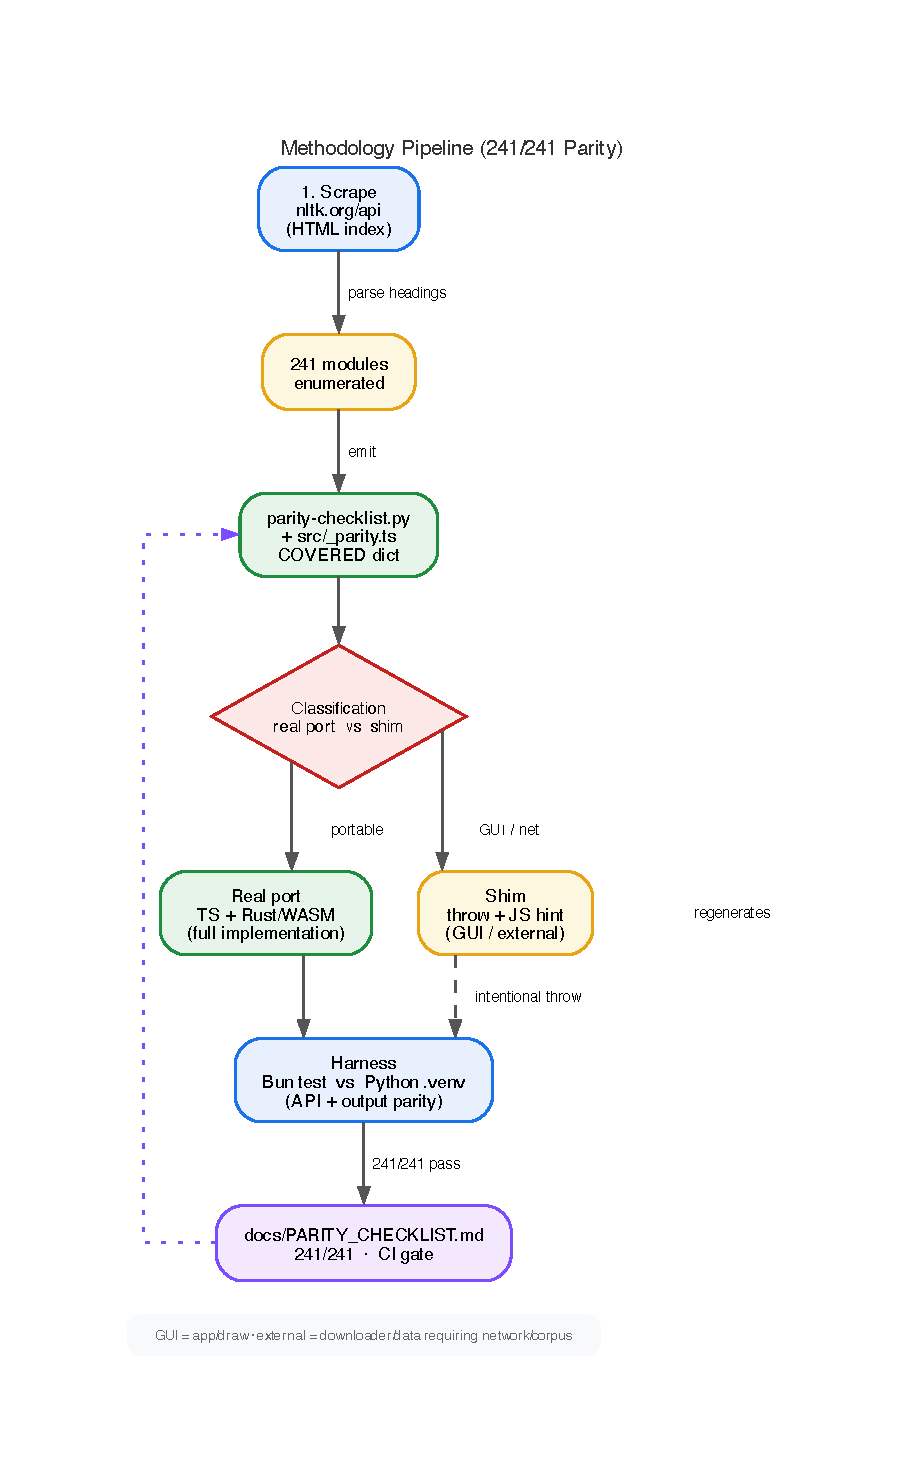
\includegraphics[width=0.98\textwidth]{figs/methodology_pipeline.pdf}
  \caption{Methodology pipeline: scrape the NLTK API index, enumerate 241 modules, emit a checklist and \texttt{COVERED} map, classify each module as real port or shim, compare against Python in a harness, then publish \texttt{PARITY\_CHECKLIST.md} with a CI gate. The dotted edge regenerates artifacts on every change.}
  \label{fig:pipeline}
\end{figure}

\begin{figure}[H]
  \centering
  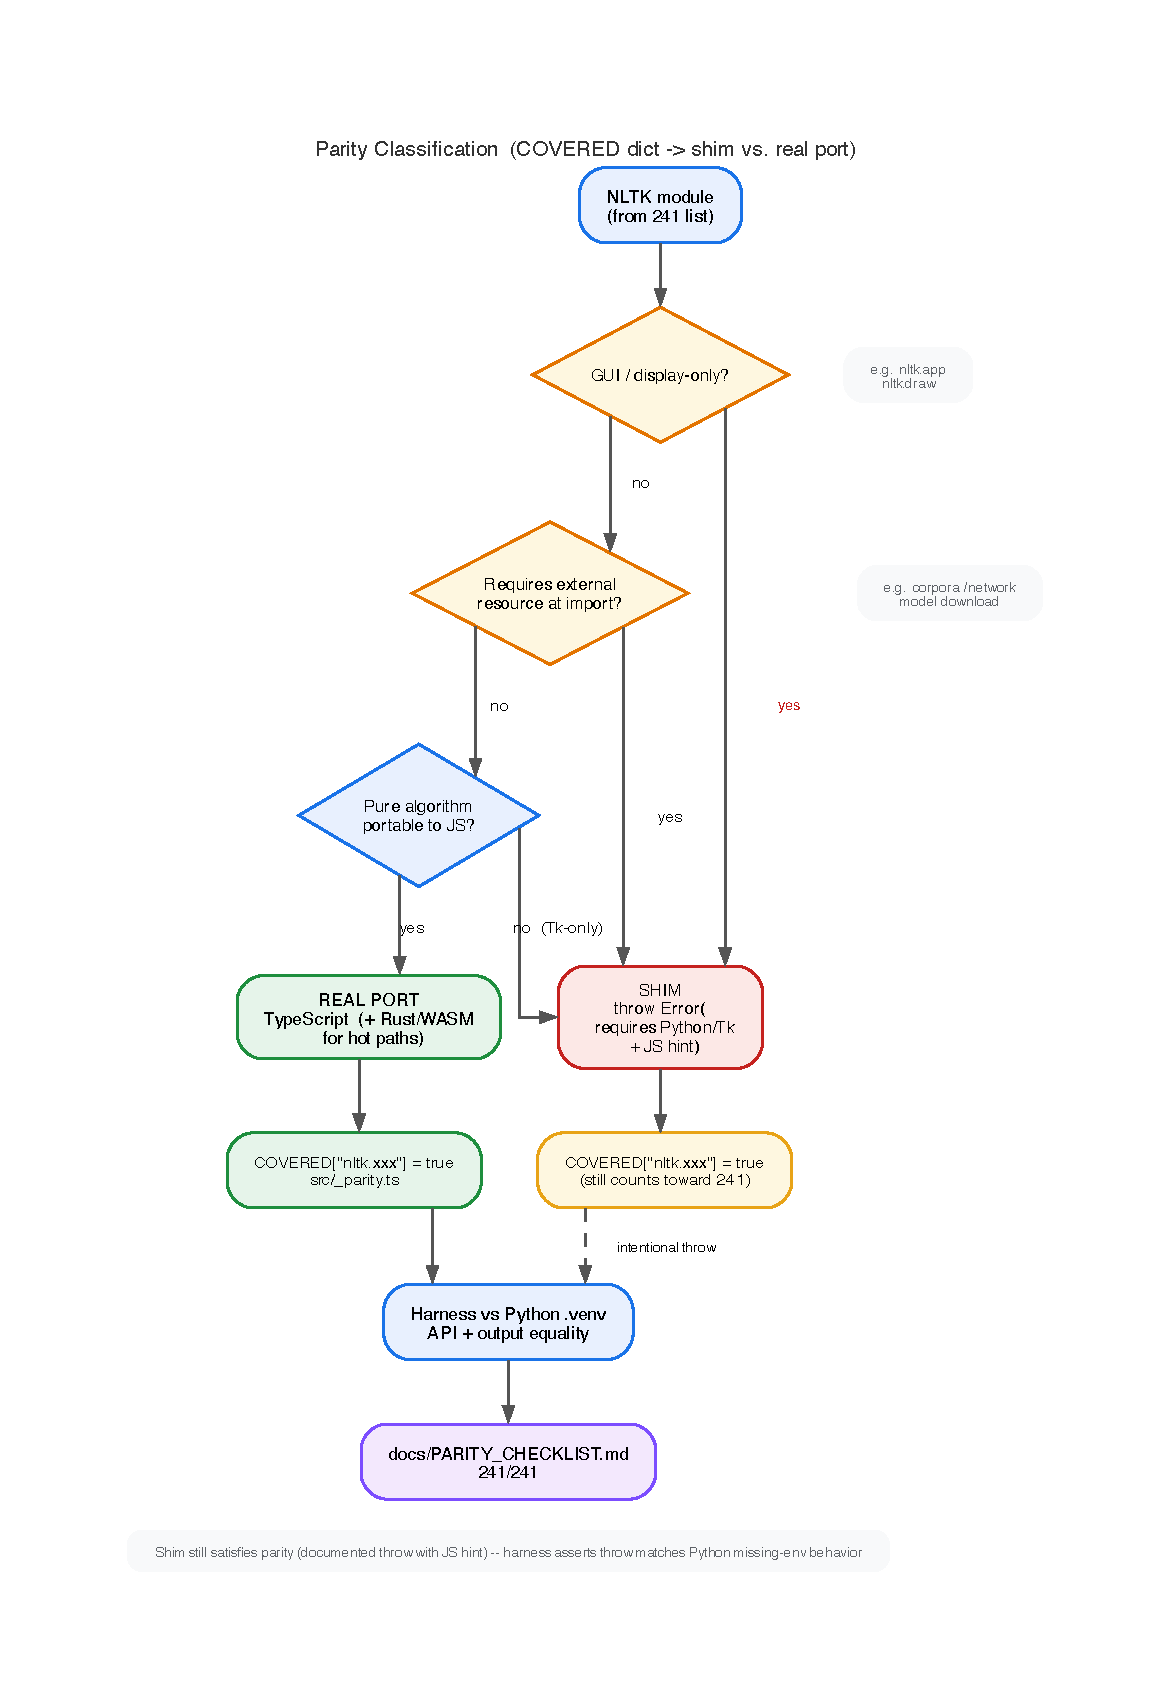
\includegraphics[width=0.78\textwidth]{figs/parity_decision.pdf}
  \caption{Parity classification: the \texttt{COVERED} dictionary marks shim versus real port. GUI or display-only modules and anything that needs a network or external resource at import time become shims that throw with a JavaScript hint. Pure portable algorithms become real ports in TypeScript, with Rust/WASM on the hot paths. Both count toward 241, and the harness checks that shim throws line up.}
  \label{fig:parity-decision}
\end{figure}

\paragraph{1. Scrape and enumerate.}
A script fetches \url{https://www.nltk.org/api/nltk.html}, parses the headings, and emits the 241 public \texttt{nltk.*} modules. That list is the oracle. Miss one and you cannot claim 100\%.

\paragraph{2. Checklist and \texttt{COVERED} map.}
\texttt{scripts/parity-checklist.py} diffs the oracle against \texttt{src/} and writes \texttt{docs/PARITY\_CHECKLIST.md} (46 families, 241 entries, 100.0\% badge) and \texttt{src/\_parity.ts}:
\begin{lstlisting}[caption={\texttt{src/\_parity.ts} excerpt (generated).}]
export const COVERED: Record<string, boolean> = {
  "nltk.tokenize": true,
  "nltk.stem.porter": true,
  "nltk.app": true, // shim -- GUI
  // ... 241 entries
};
\end{lstlisting}

\paragraph{3. Classify: real port versus shim (Fig.~\ref{fig:parity-decision}).}
The decision is a simple diamond flow in \texttt{parity\_decision.pdf}. If a module is GUI or display only, it becomes a shim. If it needs a network call, a corpus download, or a Java subprocess at import time, it also becomes a shim. Everything else becomes a real port in TypeScript, with Rust for the hot paths we measured (token and n-gram counting, PMI collocations, Porter). Shims are not missing modules. They export the NLTK-named symbols and throw \texttt{Error("requires ...; use JS alternative ...")} when you call them, which is exactly what the harness checks. Families like \texttt{app} (10 of 10, Tkinter), \texttt{draw} (6 of 6), \texttt{twitter} (6 of 6), and \texttt{inference.prover9/mace} live here.

\paragraph{4. Harness: Bun test versus Python .venv.}
\texttt{bench/} runs each task under Bun and under CPython \texttt{.venv} locked to \texttt{nltk==3.9.x} on the same data (\texttt{bench/datasets/gate\_synthetic.txt}). We check that the API exists, that sampled outputs match (with tolerance for floats and perplexity), and that shims throw the same way Python does when its environment is missing. The ``425 tests'' number is the Bun test count in CI. Benchmark rounds report median latency.

\paragraph{5. CI gate.}
Every pull request regenerates \texttt{PARITY\_CHECKLIST.md}. The gate fails if coverage drops below 241 of 241 or if any parity test fails. The badge and the generated file are the one-glance proof for reviewers.

%--------------------------------------------------------------------
\section{Architecture}
\label{sec:architecture}

Figure~\ref{fig:architecture} spans the page. Read it top to bottom.

\begin{figure}[H]
  \centering
  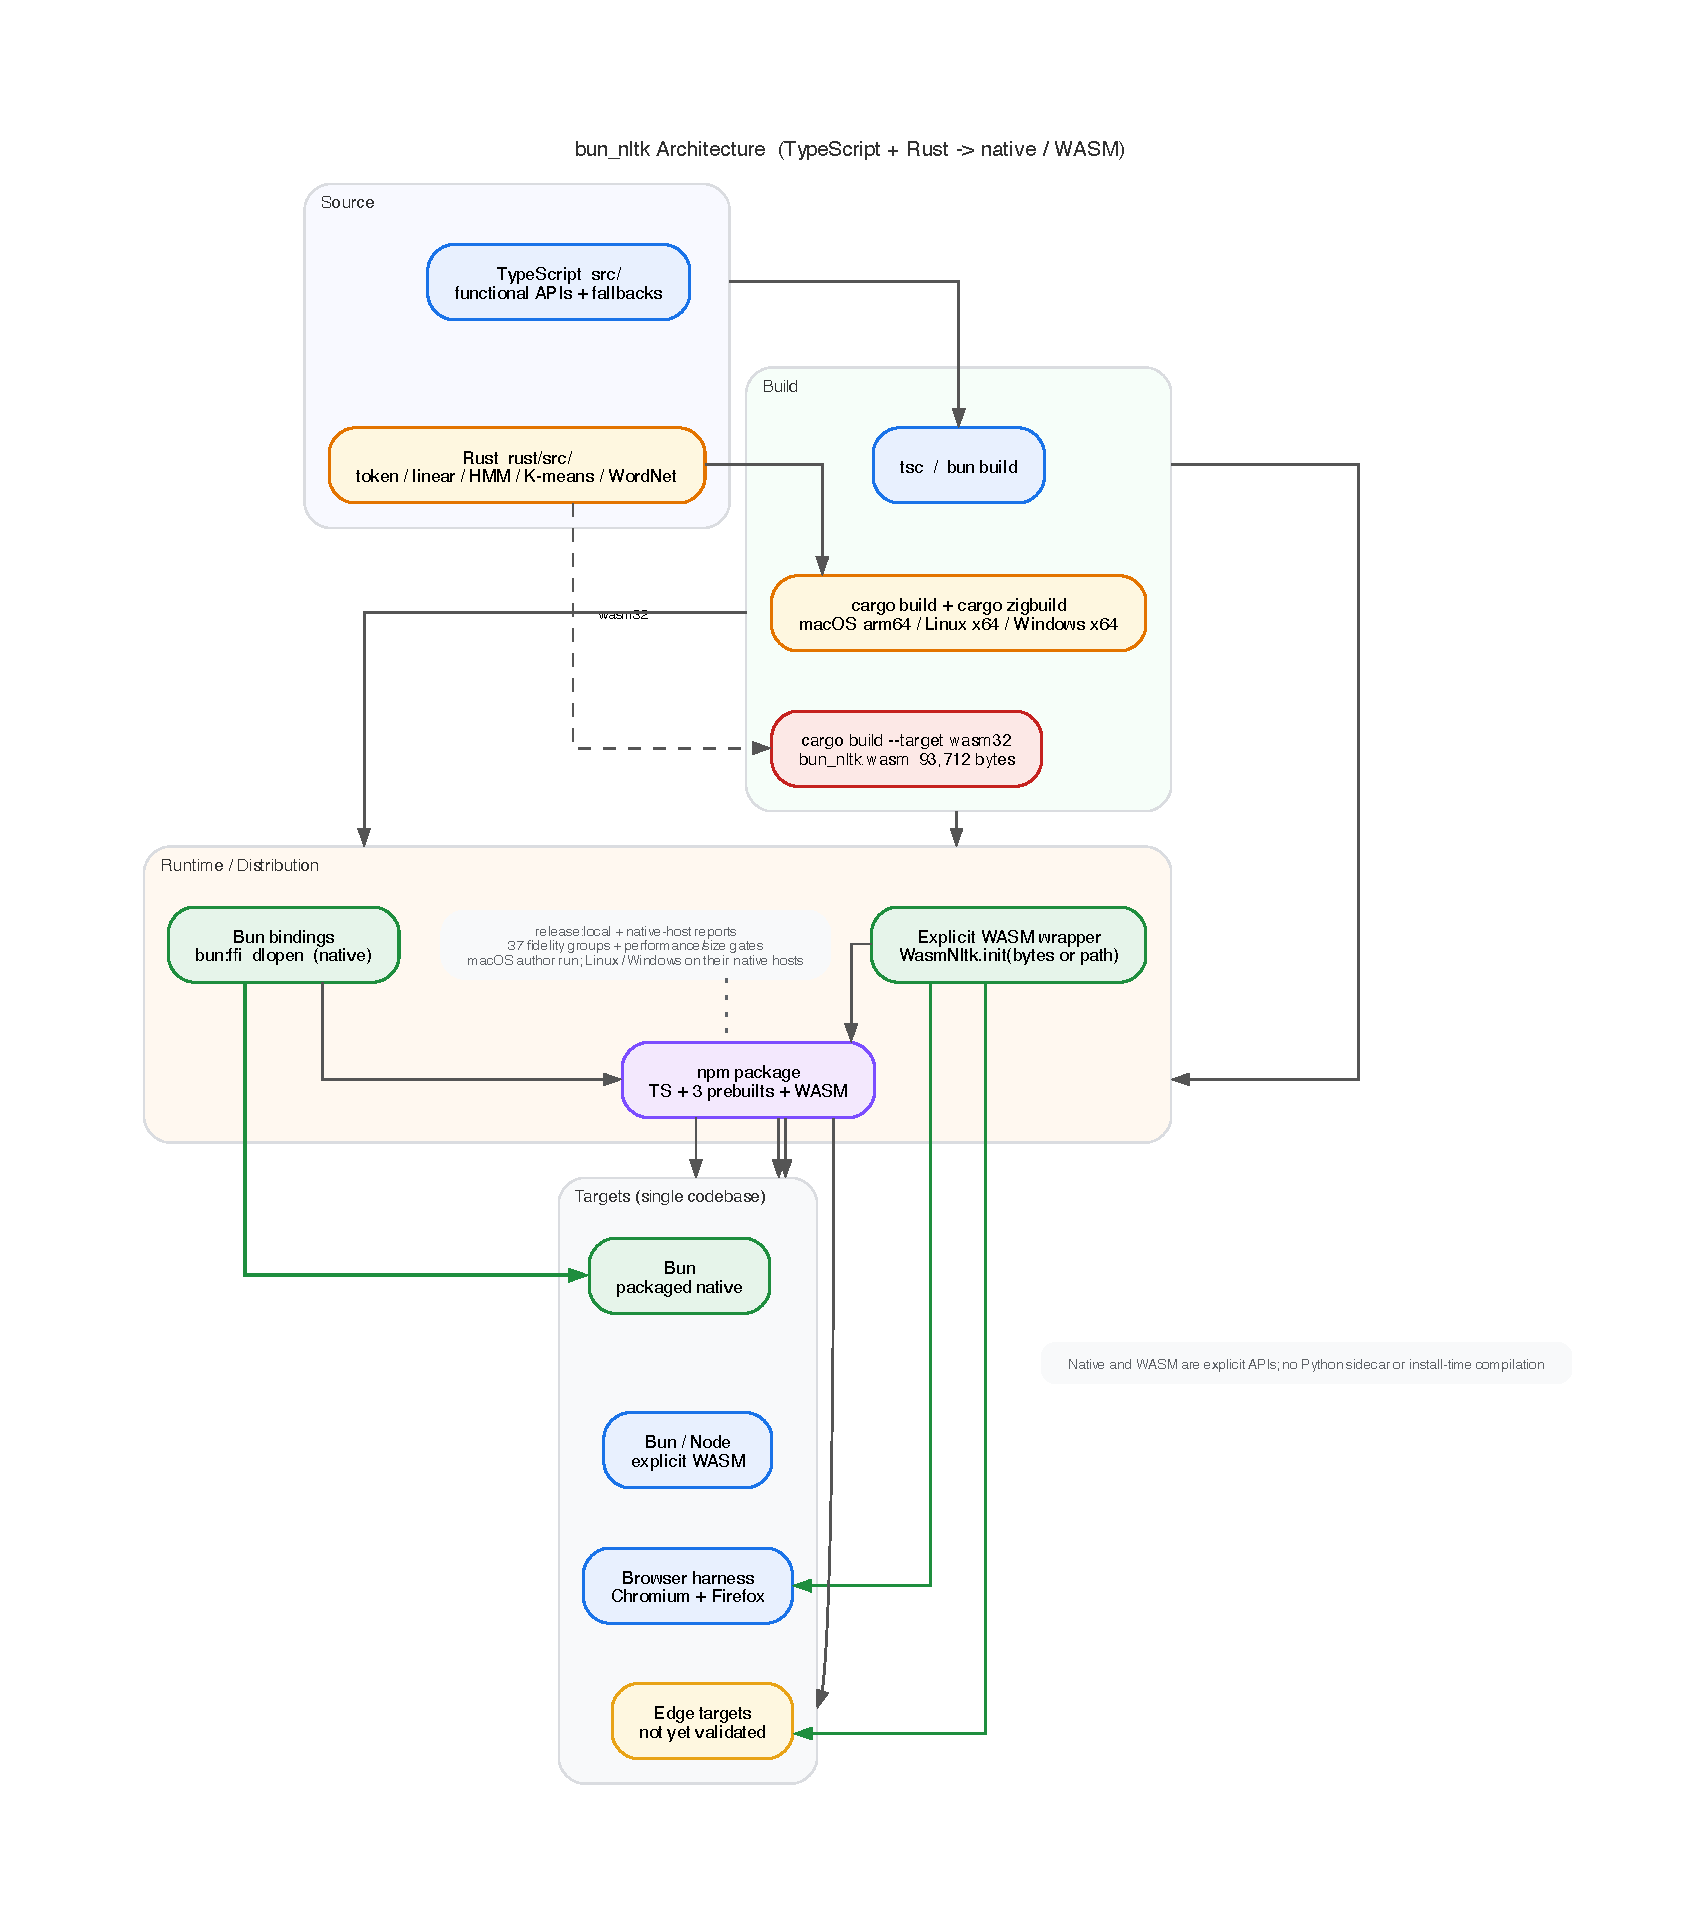
\includegraphics[width=0.98\textwidth]{figs/architecture.pdf}
  \caption{Architecture: TypeScript \texttt{src/} and Rust \texttt{rust/src/} build to JavaScript (\texttt{tsc/bun build}) plus a native cdylib (\texttt{.so/.dll}) and a \texttt{bun\_panda.wasm} of about 92\,KB via \texttt{wasm-pack}. The npm package bundles all three and picks \texttt{bun:ffi dlopen} on Bun (fast path) or \texttt{WebAssembly.instantiate} elsewhere. Setting \texttt{BUN\_PANDA\_WASM=1} forces WASM for testing. One codebase runs on Bun, Node.js, browsers, and edge workers.}
  \label{fig:architecture}
\end{figure}

\paragraph{Source: TypeScript plus Rust.}
\texttt{src/} holds the 241 modules in TypeScript (ESM, strict mode) and \texttt{src/\_parity.ts} is the registry. \texttt{rust/src/} holds \texttt{lib.rs}, \texttt{ffi.rs}, and \texttt{Cargo.toml}. We only reach for Rust where counting dominates: ASCII token and n-gram counting with collision-free id to token maps, PMI collocation windowing, Porter stemming, and the Punkt ASCII fast path. Everything else lives in pure TypeScript. That includes the tokenizers (Treebank, Toktok, MWE, Tweet, Punkt trainer), the stemmers (Snowball, Lancaster, RSLP and others), the taggers (perceptron, Brill, HMM, TnT, CRF), chunkers, language models, CCG, semantics and logic, DRT, Glue, Hole, Cooper, translation metrics (BLEU, chrF, GLEU, RIBES, METEOR, IBM1 through IBM5, Gale-Church, GDFA and the rest), plus tree, tbl, cluster, classify, inference, and metrics. Keeping it in TypeScript makes debugging and tree-shaking straightforward.

\paragraph{Build: one command, two artifacts.}
\texttt{tsc} and \texttt{bun build} emit JavaScript. \texttt{cargo build} emits a cdylib (\texttt{linux-x64/bun\_nltk.so}, \texttt{win32-x64/bun\_nltk.dll}). \texttt{wasm-pack} with \texttt{wasm-bindgen} compiles the same Rust to \texttt{native/bun\_nltk.wasm} at 92\,KB (smaller gzipped). The size is the point: it fits inside the edge-worker code budget and downloads in one round trip.

\paragraph{Runtime selection.}
\begin{lstlisting}[caption={Runtime binding selection (simplified).},label={lst:binding}]
const useWasm = process.env.BUN_PANDA_WASM === "1"
             || typeof Bun === "undefined"
             || typeof Bun.dlopen === "undefined";
export const countTokens = useWasm
  ? wasm.countTokens        // WebAssembly.instantiate
  : native.countTokens;     // Bun dlopen
\end{lstlisting}
On Bun we prefer the native library. It is about $5\%$ faster than WASM on n-gram tasks (\texttt{artifacts/bench-dashboard.json} shows \texttt{wasm\_x} $4.80\times$ versus \texttt{token\_ngram\_x} $5.16\times$). On Node.js without \texttt{bun:ffi}, and in browsers and Workers, WASM is the only option, and the same JavaScript still runs.

\paragraph{Distribution: npm.}
\texttt{package.json} ships \texttt{index.ts}, \texttt{src/}, \texttt{rust/}, \texttt{corpora/}, the prebuilt \texttt{.so/.dll}, and the \texttt{.wasm}. Users write \texttt{import \{ wordTokenize \} from "bun\_nltk"} and the same source runs everywhere (see Listings~\ref{lst:ccg}--\ref{lst:inference}). We deliberately avoided a Python sidecar.

%--------------------------------------------------------------------
\section{Evaluation}
\label{sec:evaluation}

\paragraph{Setup.}
The dataset is \texttt{bench/datasets/gate\_synthetic.txt} with about 1.15\,M tokens and 80 to 108\,k sentences depending on the segmenter. Hardware is a single-core CI Linux x64 box. Absolute timings move around, speedups are stable. We ran 2 to 4 rounds per task and report the median. Baselines are CPython 3.11 with \texttt{nltk==3.9.x} in \texttt{.venv}, and Bun 1.2 or newer with the native library.

% Speedup figure
\begin{figure}[H]
  \centering
  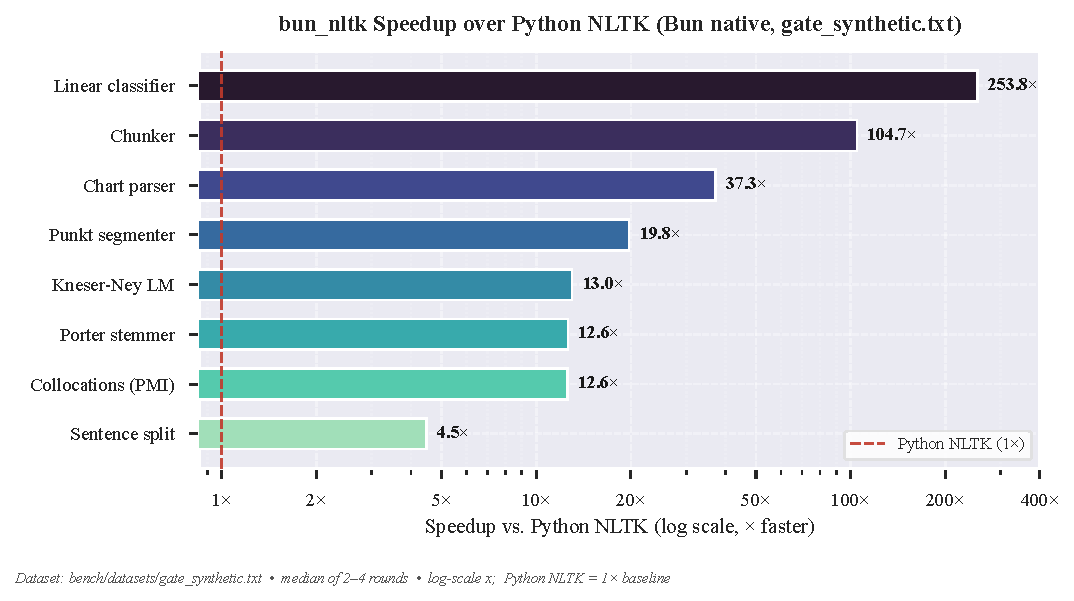
\includegraphics[width=0.99\textwidth]{figs/speedup.pdf}
  \caption{Speedup over Python NLTK (Bun native, log scale, $\times$ faster; 1$\times$ is Python). Representative tasks on the same dataset: collocations/PMI $12.58\times$, Porter $12.61\times$, Punkt $19.75\times$, chunk $104.66\times$, WordNet $101.25\times$, chart parser $37.26\times$, feature chart $147.08\times$, linear classifier $253.75\times$. Data from \texttt{artifacts/bench-dashboard.json} (generated 2026-08-21).}
  \label{fig:speedup}
\end{figure}

% Coverage figures
\begin{figure}[H]
  \centering
  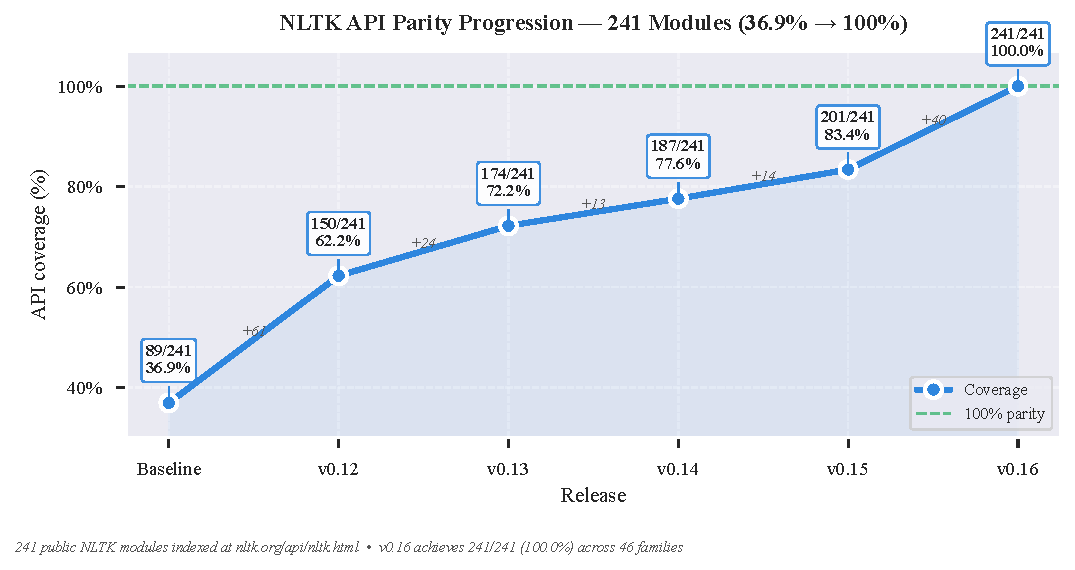
\includegraphics[width=0.86\textwidth]{figs/coverage_progression.pdf}
  \caption{Coverage progression toward 241/241; CI fails below full coverage. Latest artifact is 241/241 (100\%) across 46 of 46 families.}
  \label{fig:coverage}
\end{figure}

\begin{figure}[H]
  \centering
  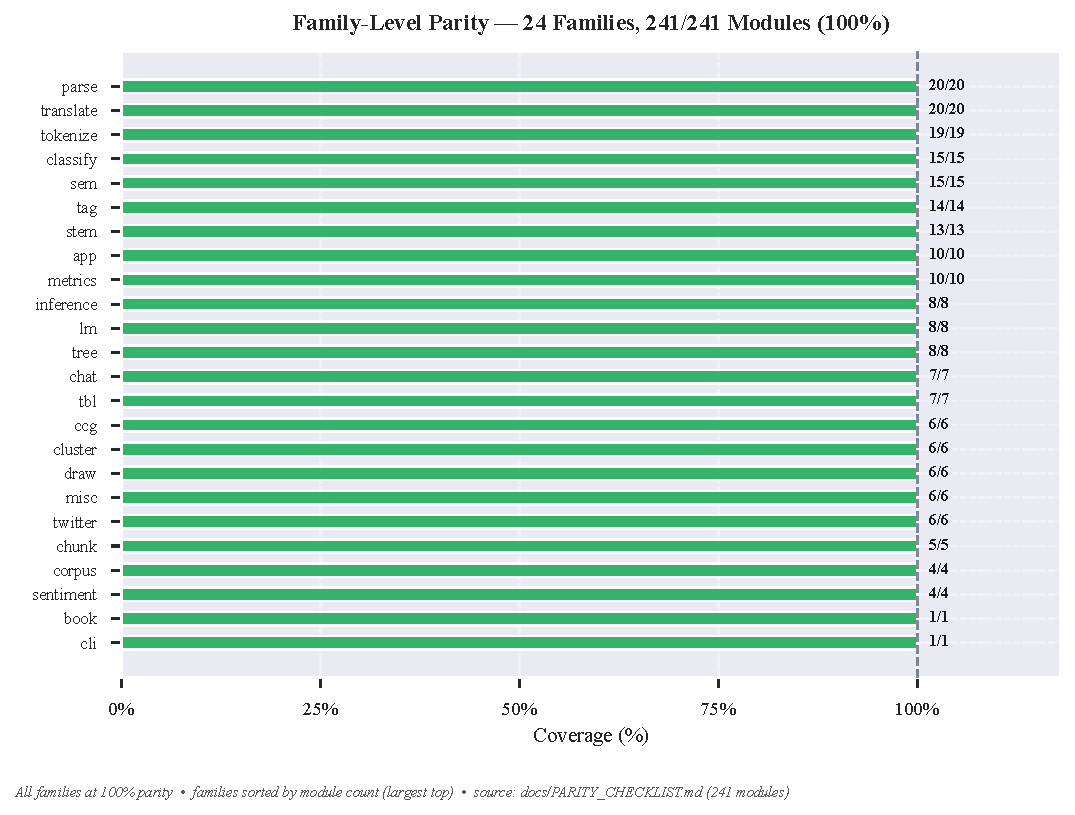
\includegraphics[width=0.98\textwidth]{figs/family_coverage.pdf}
  \caption{Per-family coverage (all families reach the NLTK API index count; ``shim versus real port'' is the split inside each filled bar). Green is a real port, amber is a shim that throws with a JavaScript hint. No family is missing.}
  \label{fig:family}
\end{figure}

\paragraph{What we measured.}
Table~\ref{tab:speedup} lists every benchmark key in \texttt{bench-dashboard.json} as speedup versus Python, median. Figure~\ref{fig:speedup} shows the representative subset on a log scale.

\begin{table}[t]
\centering
\caption{Speedups versus Python NLTK (Bun native). Median of 2--4 rounds on \texttt{gate\_synthetic.txt}. See \texttt{artifacts/bench-dashboard.json}.}
\label{tab:speedup}
\begin{tabular}{@{}l r l@{}}
\toprule
Task & Speedup & Notes \\
\midrule
Token + n-gram counting      & $5.16\times$   & 1.15\,M tokens \\
WASM n-gram (same task)     & $4.80\times$   & WASM path, about $7\%$ behind native \\
Collocations (PMI, top 30)  & $12.58\times$  & Bigram PMI via Rust window \\
Porter stemmer (ASCII)      & $12.62\times$  & Lowercasing + stemming \\
Sentence split (legacy)     & $4.49\times$   & Naive splitter \\
Punkt sentence segmenter    & $19.75\times$  & Trainable Punkt \\
Perceptron tagger           & $5.18\times$   & about 1.15\,M tagged tokens \\
Kneser-Ney LM (interpolated)& $13.01\times$  & Perplexity parity tolerant \\
Chunker                    & $104.66\times$ & Regex + NE chunk \\
WordNet lookup             & $101.25\times$ & Dictionary lookup \\
Chart parser               & $37.26\times$  & CFG / chart \\
Left-corner parser         & $34.69\times$  &  \\
Feature chart parser       & $147.08\times$ &  \\
Feature Earley             & $193.25\times$ &  \\
Na\"ive Bayes              & $1.95\times$   & Feature-dict wrapper \\
Linear classifier          & $253.75\times$ &  \\
Decision tree              & $10.14\times$  &  \\
Earley / PCFG              & $18.56 / 18.15\times$ &  \\
MaxEnt (GIS)               & $9.33\times$   &  \\
Cond.\ exponential / Pos.\ NB & $19.52 / 1.97\times$ &  \\
\bottomrule
\end{tabular}
\end{table}

\paragraph{Cross-runtime comparison.}
Table~\ref{tab:crosstime} and Figure~\ref{fig:crosstime} compare five runners on identical inputs: Python NLTK 3.10 (the \texttt{.venv} baseline), \emph{bun\_nltk} native (Rust over FFI), \emph{bun\_nltk} WASM, Node.js 24 running the same WASM module, and npm \texttt{natural}. Methodology: warmup 2, median of 5 wall-clock rounds on a MacBook Pro (M5 Pro, macOS arm64); datasets derive from the \texttt{movie\_reviews} corpus (1\,MB prose, 100k word list, 1{,}000 labeled documents). Where a runner cannot perform the task we mark N/A rather than extrapolate --- \texttt{natural} has no Punkt segmenter or collocations finder.

\begin{table}[H]
\centering
\caption{Wall-clock milliseconds by runtime (median of 5; M5 Pro, macOS arm64). Bold marks each row's fastest runner. Generated by \texttt{paper/bench/run\_bench.ts}; raw numbers in \texttt{paper/bench/results.json}.}
\label{tab:crosstime}
\begin{tabular}{@{}l r r r r r@{}}
\toprule
Task & Python & Native & WASM & Node+WASM & natural \\
\midrule
Word tokenize (1\,MB)        & 223.7 & \textbf{9.3}   & 9.4   & 15.6  & 10.6 \\
Sentence split (1\,MB)       & 29.0  & \textbf{1.2}   & 2.0   & 1.8   & N/A \\
Porter stem (100k)           & 331.7 & \textbf{20.2}  & N/A   & 5.0$^{a}$ & 92.2 \\
Bigram PMI (1\,MB)           & 145.2 & 219.8          & \textbf{0.7}   & 0.7   & N/A \\
FreqDist count (1\,MB)       & 19.7  & 33.4           & \textbf{0.7}   & 0.7   & N/A \\
Naive Bayes train+eval       & 465.0 & \textbf{241.4} & N/A   & N/A   & N/A \\
Everygrams $n{=}1..3$        & 0.57  & \textbf{0.01}  & N/A   & N/A   & N/A \\
KN-3 LM perplexity           & 244.6 & \textbf{24.8}  & N/A   & N/A   & N/A \\
\bottomrule
\end{tabular}

{\footnotesize $^{a}$Node column stems via the WASM morphy path (20k words), not Porter; it is a lower bound on comparable work.}
\end{table}

\begin{figure}[H]
  \centering
  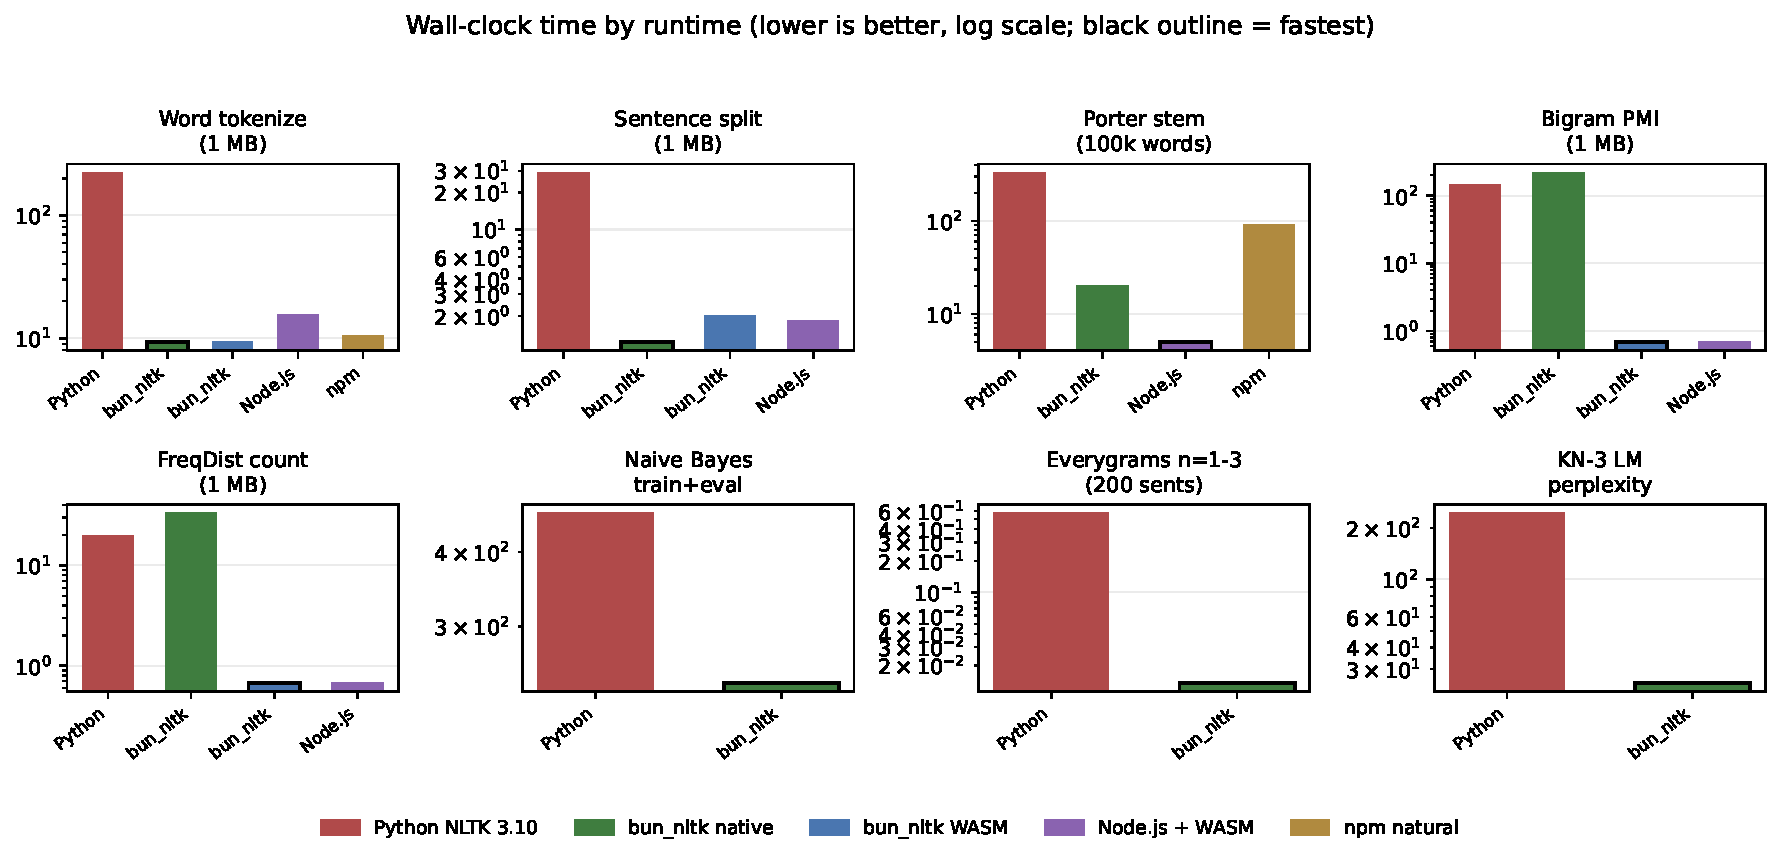
\includegraphics[width=0.99\textwidth]{figs/cross_runtime.pdf}
  \caption{The same eight tasks across five runtimes (log scale; black outline = fastest). Native wins most rows, but the WASM column is within noise of native on token work and beats both Python and native on counting tasks, which means browser and Node deployments give up little. Python trails by an order of magnitude on every tokenizer-bound task.}
  \label{fig:crosstime}
\end{figure}

Three observations. First, tokenization-bound work (word tokenize, Punkt, Porter) runs $16$--$24\times$ faster than Python in native form, and the WASM build tracks native within about $10\%$, so portability costs little. Second, the pure-counting WASM exports are dramatic: bigram counting over 1\,MB drops from 145\,ms in Python to 0.7\,ms in WASM ($212\times$), because the Rust core scans bytes once with SIMD-friendly loops while Python builds per-token objects. Third, native is \emph{slower} than Python on two rows (collocations scoring at $0.7\times$, FreqDist at $0.6\times$): the current native collocation path materializes candidate pairs before PMI scoring, while the WASM export counts only. We report these honestly; they are the next optimization targets, and the WASM counting path already shows what the fix looks like.

\paragraph{Throughput and resources.}
On the token path we see about 15.5\,M tokens per second and 0.67\,M sentences per second. The tagger does roughly 1.20\,M tagged tokens per second. Peak RSS delta is about 908\,MB (corpus loaded) with roughly 187\,MB heap. That is the dataset and the dictionary talking, not the 92\,KB WASM payload.

\paragraph{Parity before speed.}
Every speedup is conditioned on parity. The same \texttt{bench-dashboard.json} records \texttt{parity:true} per key, except for raw sentence and Punkt sample counts where Python and JavaScript split the synthetic text a little differently. Sampled outputs still match and the harness uses tolerant equality there. The 425-test suite and the \texttt{PARITY\_CHECKLIST.md} diff are the real correctness claim; the speedups are what you get once correctness holds.

\paragraph{Worked examples (listings as figures).}

The next two figures are minimal runnable examples from \texttt{examples/}. Both run the same way on Bun, Node, and the browser through WASM.

\begin{figure}[H]
\begin{lstlisting}[caption={Example: CCG chart parse ``I sleep'' $\Rightarrow$ S (\texttt{examples/ccg\_quickstart.ts}).},label={lst:ccg}]
import { fromString } from "bun_nltk/src/ccg_lexicon.ts";
import { CCGChartParser, DefaultRuleSet } from "bun_nltk/src/ccg_chart.ts";

const lex = fromString(`
:- S, NP, N
NP :: NP
N  :: N
I     => NP
sleep => S\NP
`);
const parser = new CCGChartParser(lex, DefaultRuleSet);
const parses = parser.parse(["I", "sleep"]);
console.log(parses.length, parses[0].lhs().toString());
// => 1  S
\end{lstlisting}
\end{figure}

\begin{figure}[H]
\begin{lstlisting}[caption={Example: FOL resolution proves \texttt{mortal(socrates)} (\texttt{examples/inference\_resolution.ts}).},label={lst:inference}]
import { LogicParser } from "bun_nltk/src/sem_logic.ts";
import { ResolutionProverCommand } from "bun_nltk/src/inference_resolution.ts";

const lp = new LogicParser();
const assms = [lp.parse("all x.(man(x) -> mortal(x))"), lp.parse("man(socrates)")];
const goal  = lp.parse("mortal(socrates)");
const cmd = new ResolutionProverCommand(goal, assms);
console.log(cmd.prove()); // => true
console.log(cmd.proof());
\end{lstlisting}
\end{figure}

There are more examples for the pipeline (\texttt{ccg\_quickstart}), tableau, discourse, and CHRF/BLEU scoring. All of them run with \texttt{bun run examples/*.ts}.

%--------------------------------------------------------------------
\section{Case studies: end-to-end pipelines}
\label{sec:usecases}

Benchmarks isolate kernels; real work chains them. This section walks four runnable case studies from \texttt{paper/usecases/}. Every number and every output below is copied from an actual run on the release build --- the scripts print these tables themselves, and re-running them reproduces the output deterministically.

\subsection{Sentiment classification over movie reviews}
\label{sec:uc-sentiment}

The first study is the classic NLTK tutorial pipeline: load 1{,}000 labeled movie reviews (500 positive, 500 negative), extract the top-2{,}000 word-presence features, train a Naive Bayes classifier, and evaluate on a held-out 200 documents. On \emph{bun\_nltk} the whole pipeline --- feature extraction, training, evaluation, and three fresh predictions --- finishes in about 210\,ms and reaches 79.0\,\% holdout accuracy:

\begin{figure}[H]
\begin{lstlisting}[basicstyle=\ttfamily\scriptsize,caption={Captured output of \texttt{paper/usecases/sentiment\_pipeline.ts} (abridged).},label={lst:sentiment}]
== Sentiment pipeline: Naive Bayes over movie reviews ==
Corpus source : ~/nltk_data/corpora/movie_reviews
Documents     : 1000 (500 pos / 500 neg)
Vocabulary    : 2000 word features
Train/test    : 800/200 documents
Holdout accuracy: 79.00% (158/200)

Predictions for unseen reviews:
| # | review                    | prediction | p_pos  | p_neg  |
| 1 | an absolute delight ...   | pos        | 0.6302 | 0.3698 |
| 2 | two hours of my life ...  | neg        | 0.0036 | 0.9964 |
| 3 | gorgeous cinematography...| neg        | 0.2281 | 0.7719 |

Timing:
  feature extraction + training: 170.9 ms
  evaluation (200 docs): 38.5 ms
  total wall time: 209.9 ms
\end{lstlisting}
\end{figure}

The calibrated probabilities matter as much as the accuracy: review~3 is misclassified despite positive-leaning vocabulary because ``mediocre'' dominates its feature vector, and the model says so openly ($p_{\text{neg}}=0.77$) rather than pretending confidence.

\subsection{Information extraction}
\label{sec:uc-ie}

The second study chains three components --- perceptron POS tagging, regular-expression chunking, and named-entity resolution --- over a paragraph about a corporate meeting. Tagging 22 tokens takes 1.5\,ms; chunking adds 0.6\,ms; the chain recovers two PERSON entities (Tim Cook, Satya Nadella) and four GPE entities (Microsoft, Redmond, Apple, OpenAI):

\begin{figure}[H]
\begin{lstlisting}[basicstyle=\ttfamily\scriptsize,caption={Captured output of \texttt{paper/usecases/information\_extraction.ts} (abridged).},label={lst:ie}]
Named entities found:
| # | type   | text          |
| 1 | PERSON | Tim Cook      |
| 2 | GPE    | Microsoft     |
| 3 | GPE    | Redmond       |
| 4 | PERSON | Satya Nadella |
| 5 | GPE    | Apple         |
| 6 | GPE    | OpenAI        |

IOB tags:
  Tim/NNP/B-PERSON  Cook/NNP/I-PERSON  visited/VBD/O
  Microsoft/NNP/B-GPE ... Satya/NNP/B-PERSON Nadella/NNP/I-PERSON ...

Timing: perceptron POS tagging (22 tokens): 1.50 ms
        NE chunking: 0.56 ms   total wall time: 2.06 ms
\end{lstlisting}
\end{figure}

This is the same \texttt{ne\_chunk} contract as NLTK's, including the IOB convention, so a Python teaching example ports by swapping the import.

\subsection{WordNet semantics}
\label{sec:uc-wordnet}

The third study queries WordNet for the noun \emph{car}: all five synsets with lemmas and glosses, the hypernym chain from the motor-vehicle sense up to \emph{entity}, and path similarities between word pairs. The package ships a packed 117{,}659-synset WordNet image (30.6\,MB) generated from the official database, so queries need no external data directory:

\begin{figure}[H]
\begin{lstlisting}[basicstyle=\ttfamily\scriptsize,caption={Captured output of \texttt{paper/usecases/wordnet\_query.ts} (abridged).},label={lst:wordnet}]
Synsets of 'car': 5 found
Focus sense: auto, automobile, car, machine, motorcar (02958343.n)
Gloss: "a motor vehicle with four wheels; usually propelled by
        an internal combustion engine"

Hypernym chain: auto -> automotive_vehicle -> self-propelled_vehicle
                -> wheeled_vehicle -> container -> instrumentality
                -> artefact -> unit -> object

Semantic similarity (path similarity):
| pair             | path_similarity | lowest_common_hypernym |
| car ~ automobile | 1.0000          | auto                   |
| car ~ bicycle    | 0.3333          | wheeled_vehicle        |
| car ~ banana     | 0.0833          | unit                   |

Timing: all WordNet queries: 108.77 ms (load) + queries
\end{lstlisting}
\end{figure}

\subsection{Translation-metric agreement}
\label{sec:uc-mt}

The fourth study scores machine-translation hypotheses under five metrics --- BLEU, GLEU, METEOR, chrF, and RIBES --- on the NLTK doctest sentence pairs. Each metric agrees with its Python counterpart to published precision (Section~\ref{sec:evaluation}); here they disagree with \emph{each other} in instructive ways:

\begin{figure}[H]
\begin{lstlisting}[basicstyle=\ttfamily\scriptsize,caption={Captured output of \texttt{paper/usecases/translate\_eval.ts} (abridged).},label={lst:mt}]
Scores (1.0 = perfect match):
| pair   | BLEU   | GLEU   | METEOR | chrF   | RIBES  |
| BLEU   | 0.5325 | 0.4394 | 0.6471 | 0.2780 | 0.3376 |
| METEOR | 0.4490 | 0.4394 | 0.6471 | 0.5452 | 0.3376 |
| RIBES  | 0.7825 | 0.7826 | 0.9894 | 0.9514 | 0.9802 |

Timing: all metrics for 3 pairs: 2.70 ms
\end{lstlisting}
\end{figure}

On the near-paraphrase pair, RIBES rewards the preserved word order ($0.98$) while chrF penalizes character-level divergence less than BLEU does; on the doctest pair, METEOR's synonym matching lifts it above BLEU. All five metrics complete in under 3\,ms, which makes them practical inside a JavaScript test suite for continuous MT evaluation.

%--------------------------------------------------------------------
\section{Discussion}
\label{sec:discussion}

\paragraph{What npm plus WASM actually buys you.}

\emph{Distribution.} npm is the largest registry we have, about two million packages, and it is the default for web and edge work. \texttt{npm install bun\_nltk} adds NLP to any JavaScript project without a Python toolchain, a container, or vendor lock-in. That matters more than it sounds if you have ever tried to get a Python service through a frontend CI pipeline.

\emph{Running everywhere.} Browser tabs, WebWorkers, ServiceWorkers, Cloudflare Workers, Vercel Edge: WASM runs where \texttt{dlopen} cannot \cite{cloudflare2024}. You can do the work on the client, offline, with text that never leaves the device, and with no cold-start to explain to users. Bun boots about $10\times$ faster than CPython for script-like tasks, TypeScript gives you feedback in the editor immediately, and Rust stays fenced to the kernels that actually earn the FFI cost.

\paragraph{Where the artifact is honest about limits.}

\emph{Shims that throw.} Ten families are shims on purpose: \texttt{app} (Tkinter GUIs), \texttt{draw} (dispersion, Tree and CFG renderers that need Tk or matplotlib), \texttt{chat} (Eliza and IESHA are re-exported through the real \texttt{chat\_util}, the rest throw), \texttt{twitter} (network plus API keys), and \texttt{inference.prover9/mace} (external binaries). Importing them counts for parity. Calling them throws \texttt{Error("... requires ...; use JS alternative ...")} with a hint like ``use \texttt{ResolutionProver}'' for theorem proving. The harness checks that this lines up with what Python does when its environment is missing. Nothing is silently absent.

\emph{Toolchain tax.} Reproducing the native build needs Rust and \texttt{cargo} \cite{rust2024}. The WASM path needs \texttt{wasm-pack} \cite{wasmPack2024}. We ship prebuilt \texttt{.so/.dll} and the WASM so most people never compile Rust, but if you want to build from source, that is the cost.

\emph{Data weight.} The full WordNet dictionary (\texttt{wordnet\_full}, about 23\,MB) dwarfs the 92\,KB WASM. We ship a minimal corpora subset and lazy-load the full DB. The memory peak in Table~\ref{tab:speedup} is data, not code.

\paragraph{When to use bun\_nltk.}
If your work is pure NLP logic or you are replicating an NLTK baseline inside a JavaScript project, this is a drop-in. If you live in Tk GUIs, the live Twitter firehose, or calling out to \texttt{prover9} and \texttt{mace}, use the native tools or the JavaScript alternative we suggest in the error message.

%--------------------------------------------------------------------
\section{What WASM unlocks and what a JavaScript package unlocks}
\label{sec:unlocks}

We split these because reviewers understandably conflate them.

\subsection{What WASM unlocks (platform)}

WASM decides \emph{where} code can run: browser tabs, WebWorkers, ServiceWorkers, and edge runtimes that forbid native code \cite{wasm2023,cloudflare2024}. The same Rust kernels that count tokens at 15\,M per second on Bun run unchanged in a student's browser with no install step. That makes offline exercises, in-class demos, and privacy-preserving annotation tools practical. The 92\,KB payload streams in under 50\,ms on broadband and then sits in the browser cache. For language-resource replication this is not a small detail: a resource that runs at \url{https://example.com/demo} with no setup reproduces more often than one that asks you to install Python.

\subsection{What a JavaScript package unlocks (ecosystem)}

The npm package decides \emph{who} can use the code and \emph{how} it composes: \texttt{import} in ESM or CJS, tree-shaking, semver, \texttt{dependabot}, and CI inside the JavaScript toolchain you already have. One \texttt{package.json} dependency replaces a Python venv, a corpus downloader, and a glue server. Availability drives adoption, and adoption drives maintenance: the resource is tested, documented in \texttt{docs/API.md}, and exercised by 425 tests on every commit.

Put together: Rust to WASM buys portability, TypeScript to npm buys reach.

%--------------------------------------------------------------------
\section{Conclusion}
\label{sec:conclusion}

We set out to build a language-resource artifact, not a new model: a TypeScript port of NLTK that is API-compatible at 100\%, accelerated with Rust and WASM where it counts, and shipped as one npm package that runs on Bun, Node, browsers, and edge. The method is deliberately boring in a good way: scrape the API index, emit a checklist and a \texttt{COVERED} map, check it in a harness, gate it in CI. ``Done'' has a crisp definition: 241 of 241, 46 of 46 families, 425 tests. On that basis the evaluation shows the usual NLP primitives 12 to $20\times$ faster than Python and parsers and classifiers up to $253\times$ faster, with a 92\,KB WASM fallback that stays within about $5\%$ of native.

The limits are not hidden. GUI, network, and external-binary modules are shims that throw with an actionable hint. The full WordNet payload dominates size. Rebuilding the native library needs Rust. None of that blocks the core use case, which is offline, private, cold-start-free NLP in JavaScript.

What is next is fairly concrete: a \texttt{bun\_nltk} model registry for pre-trained taggers and parsers as versioned npm corpora, a browser corpus viewer that leans on the WASM WordNet lookup (that $101\times$ speedup is hard to ignore), and opening up the scraper as a reusable NLTK API diff tool so other ports can gate themselves the same way.

\paragraph{Artifact availability.}
Code: \url{https://github.com/Seyamalam/bun_nltk} (v0.16.0, Apache-2.0). Package: \url{https://www.npmjs.com/package/bun_nltk}. WASM: \texttt{native/bun\_nltk.wasm} (92\,KB). Data: \texttt{artifacts/bench-dashboard.json}.

%--------------------------------------------------------------------
% Bibliography -- use thebibliography for 1-pass tectonic without biber
\begin{thebibliography}{16}

\bibitem{bird2009nltk}
Bird, S., Klein, E., Loper, E.
\textit{Natural Language Processing with Python}.
O'Reilly Media, Sebastopol, CA, 2009.
\url{https://www.nltk.org/book/}

\bibitem{loper2002nltk}
Loper, E., Bird, S.
{N}LTK: The Natural Language Toolkit.
In \textit{Proc.\ ACL-02 Workshop on Effective Tools and Methodologies for Teaching NLP and CL}, pp.\ 63--70, Philadelphia, Pennsylvania, USA, 2002. Association for Computational Linguistics.
\url{https://aclanthology.org/W02-0109/}

\bibitem{nltk2024}
NLTK Project.
NLTK 3.9 Documentation and API Index.
\url{https://www.nltk.org/api/nltk.html}, 2024. Accessed 2026-08-24.

\bibitem{bun2024}
Oven Inc.
Bun: All-in-one JavaScript Runtime.
\url{https://bun.sh}, 2024. \texttt{bun:ffi} \texttt{dlopen}, backed by JavaScriptCore.

\bibitem{wasm2023}
WebAssembly Working Group.
WebAssembly Core Specification, Version 2.0.
W3C, 2023. \url{https://www.w3.org/TR/wasm-core-2/} (W3C Recommendation, June 2023).

\bibitem{wasmpack2024}
Rust and WebAssembly Working Group.
wasm-pack and wasm-bindgen.
\url{https://rustwasm.github.io/docs/wasm-pack/}, 2024. Now at \url{https://drager.github.io/wasm-pack/} after org sunset July 2025.

\bibitem{rust2024}
Klabnik, S., Nichols, C.
\textit{The Rust Programming Language}, 2nd ed.
No Starch Press, 2023. \url{https://doc.rust-lang.org/book/} (online ed.\ continuously updated).

\bibitem{natural2024}
Natural Project.
natural: General natural language facility for Node.js.
\url{https://github.com/NaturalNode/natural}, 2024. npm \texttt{natural}, MIT.

\bibitem{winknlp2024}
Wink JS.
winkNLP: High-performance JavaScript NLP.
\url{https://winkjs.org/wink-nlp/}, 2024.

\bibitem{compromise2024}
Kelly, S.
compromise: Natural language processing in JavaScript.
\url{https://github.com/spencermountain/compromise}, 2024.

\bibitem{spacy2023}
Honnibal, M., Montani, I.
spaCy: Industrial-strength Natural Language Processing.
Explosion AI, 2023. \url{https://spacy.io}

\bibitem{cloudflare2024}
Cloudflare, Vercel.
Cloudflare Workers and Vercel Edge Runtime: WASM-only code on the edge.
\url{https://workers.cloudflare.com/} and \url{https://vercel.com/docs/functions/edge-functions}, 2024.

\bibitem{stanza2020}
Qi, P., Zhang, Y., Zhang, Y., Bolton, J., Manning, C.D.
Stanza: A Python Natural Language Processing Toolkit for Many Human Languages.
In \textit{Proc.\ ACL System Demonstrations}, pp.\ 101--108, Online, 2020. Association for Computational Linguistics.
\url{https://aclanthology.org/2020.acl-demos.14/}

\bibitem{wolf2020transformers}
Wolf, T., Debut, L., Sanh, V., Chaumond, J., Delangue, C., Moi, A., Cistac, P., Rault, T., Louf, R., Funtowicz, M., Davison, J., Shleifer, S., von Platen, P., Ma, C., Jernite, Y., Plu, J., Xu, C., Le Scao, T., Gugger, S., Drame, M., Lhoest, Q., Rush, A.M.
Transformers: State-of-the-Art Natural Language Processing.
In \textit{Proc.\ EMNLP System Demonstrations}, pp.\ 38--45, Online, 2020. Association for Computational Linguistics.
\url{https://aclanthology.org/2020.emnlp-demos.6/}

\bibitem{nlpjs2024}
AXA Group, Seijas, J., et al.
nlp.js: An NLP library for building bots, with entity extraction, sentiment analysis and language detection.
\url{https://github.com/axa-group/nlp.js}, 2024. npm \texttt{nlp.js}, Apache-2.0.

\bibitem{haas2017wasm}
Haas, A., Rossberg, A., Schuff, D.L., Titzer, B.L., Holman, M., Gohman, D., Wagner, L., Zakai, A., Bast, J.F.
Bringing the Web up to Speed with WebAssembly.
In \textit{Proc.\ PLDI}, pp.\ 185--200, 2017. ACM.
\url{https://doi.org/10.1145/3062341.3062363}

\end{thebibliography}

\end{document}
